\subsection*{El Modelo de las cinco fuerxas de Porter}

El Análisis Porter de las cinco fuerzas es un modelo elaborado por el economista Michael Porter en 1979,
en que se describen las 5 fuerzas que influyen en la estrategia competitiva de una compañía que determinan
las consecuencias de rentabilidad a largo plazo de un mercado, o algún segmento de éste. Las primeras cuatro
fuerzas se combinan con otras variables para crear una quinta fuerza, el nivel de competencia en una industria.

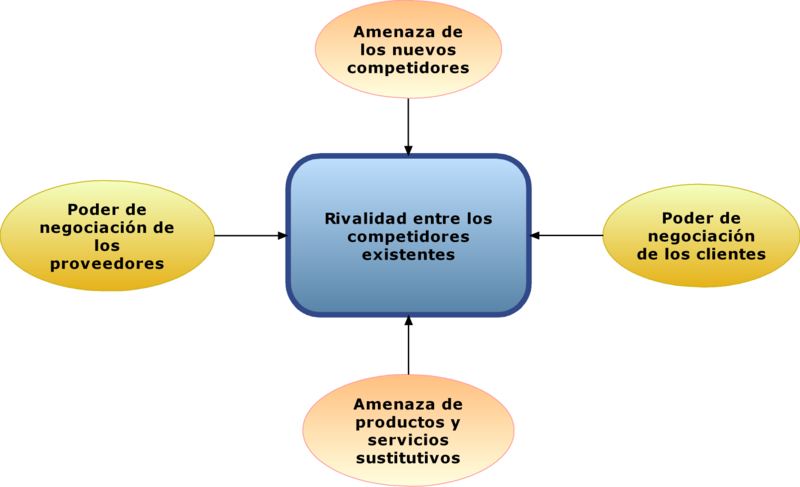
\includegraphics[height=8cm]{images/cincoFuerzas}

\begin{enumerate}
	\item \emph{Entrada Potencial de Nuevos Competidores}
		El mercado o el segmento no son atractivos dependiendo de si las barreras de entrada son fáciles
		o no de franquear por nuevos participantes, que puedan llegar con nuevos recursos y capacidades
		para apoderarse de una porción del mercado.
	\item \emph{Rivalidad entre Empresas Competidoras}
		Para una corporación será más difícil competir en un mercado o en uno de sus segmentos donde los
		competidores estén muy bien posicionados, sean muy numerosos y los costos fijos sean altos, pues
		constantemente estará enfrentada a guerras de precios, campañas publicitarias agresivas, promociones
		y entrada de nuevos productos
	\item \emph{Poder de Negociación de los Proveedores}
		Un mercado o segmento del mercado no será atractivo cuando los proveedores estén muy bien organizados
		gremialmente, tengan fuertes recursos y puedan imponer sus condiciones de precio y tamaño del pedido.
		La situación será aún más complicada si los insumos que suministran son claves para nosotros, no tienen
		sustitutos o son pocos y de alto costo. La situación será aún más crítica si al proveedor le conviene
		estratégicamente integrarse hacia delante.
	\item \emph{Poder de Negociación de los Consumidores}
		Un mercado o segmento no será atractivo cuando los clientes están muy bien organizados, el producto
		tiene varios o muchos sustitutos, el producto no es muy diferenciado o es de bajo costo para el cliente,
		lo que permite que pueda hacer sustituciones por igual o a muy bajo costo. A mayor organización de los
		compradores, mayores serán sus exigencias en materia de reducción de precios, de mayor calidad y servicios
		y por consiguiente la corporación tendrá una disminución en los márgenes de utilidad. La situación se hace
		más crítica si a las organizaciones de compradores les conviene estratégicamente sindicalizarse.
	\item \emph{Desarrollo Potencial de Productos Sustitutos}
		Un mercado o segmento no es atractivo si existen productos sustitutos reales o potenciales. La situación
		se complica si los sustitutos están más avanzados tecnológicamente o pueden entrar a precios más bajos
		reduciendo los márgenes de utilidad de la corporación y de la industria.
\end{enumerate}

\subsection*{Porter y la competitivida}

La competitividad debe ser entendida como la capacidad que tiene una organización, pública o privada, lucrativa o no, de
obtener y mantener ventajas comparativas que le permitan alcanzar, sostener y mejorar una determinada posición en el entorno
socioeconómico. El término competitividad es muy utilizado en los medios empresariales, teniendo incidencia en la forma de
plantear y desarrollar cualquier iniciativa de negocios, lo que provoca, obviamente una evolución en el modelo de empresa y
empresario.

La ventaja comparativa o competitiva de una empresa estaría en su habilidad, recursos, conocimientos y atributos, etc., de los
que dispone, y los mismos de los que carecen sus competidores o tienen en menor medida, haciendo esto posible la obtención de
unos rendimientos superiores a los de aquellos. El concepto de competitividad nos hace pensar en la idea “excelencia”, con
características de eficiencia y eficacia de la organización.

Las empresas competitivas son aquellas capaces de ofrecer continuamente productos y servicios con atributos apreciados por sus
clientes. A este conjunto de características que distinguen al producto de una empresa de sus competidores lo denominamos
ventajas competitivas. Lo único seguro acerca de las ventajas competitivas es su dinamismo; los mercados pueden cambiar sus
exigencias o la tecnología de la empresa puede verse desplazada por las de la competencia. Si una empresa no invierte en
mantenerlas, renovarlas, tarde o temprano estará condenada a perderlas.

Existen dos categorías de ventajas competitivas: de costes y de valor añadido. Las ventajas de costes están asociadas con la
capacidad de ofrecer a los clientes un producto al mínimo coste. Las ventajas competitivas de valor; por su parte, están
basadas en la oferta de un producto o servicio con atributos únicos, discernibles por los clientes, que distinguen a un
competidor de los demás. (Julián Villalba)

Michael Porter afirmaba que la competitividad está determinada por la productividad, definida como el valor del producto
generado por una unidad de trabajo o de capital. Para hablar de competitividad, continúa Porter, habría que irse a la empresa,
y al sector, e identificar cuáles son los factores que determinan que las empresas generen valor añadido y que ese valor se
venda en el mercado, y si realmente esos factores son sostenibles en el mediano y largo plazo.

Asimismo, Michael Porter establece cuatro factores que pueden ser determinantes en la competitividad:
\begin{enumerate}
	\item La dotación del país, en términos de cantidad y calidad de los factores productivos básicos (fuerza de trabajo,
		recursos naturales, capital e infraestructura), así como de las habilidades, conocimientos y tecnologías
		 especializados que determinan su capacidad para generar y asimilar innovaciones.
	\item La naturaleza de la Demanda Interna en relación con la oferta del aparato productivo nacional; en particular,
		es relevante la presencia de demandantes exigentes que presionan a los oferentes con sus demandas de artículos
		innovadores y que se anticipen a sus necesidades.
	\item La existencia de una estructura productiva conformada por empresas de distintos tamaños, pero eficientes en escala
		internacional, relacionadas horizontal y verticalmente, que aliente la competitividad mediante una oferta interna
		especializada de insumos, tecnologías y habilidades para sustentar un proceso de innovación generalizable a lo
		largo de cadenas productivas.
	\item Las condiciones prevalecientes en el país en materia de creación, organización y manejo de las empresas
\end{enumerate}

\subsection*{Arquitectura de la Empresa}

Arquitectura de la Empresa es el conjunto de elementos organizacionales (objetivos estratégicos, departamentos, procesos, tecnología,
personal, etc.) que describen a la empresa y se relacionan entre sí garantizando la alineación desde los niveles más altos (estratégicos)
hasta los más bajos (operativos), con el fin de optimizar la generación de productos y servicios que conforman la propuesta de valor
entregada a los clientes.

De esta definición destaca el hecho de que se busca una alineación de los niveles más altos con los más bajos de la empresa. Esto es
importante, debido a que todas las áreas de la empresa deben actuar en armonía para conseguir los objetivos definidos por la misma.
Esto suena muy obvio, pero en la práctica es frecuente perder este enfoque. La Arquitectura de la Empresa ayuda a conservar la
perspectiva y a garantizar esta alineación. Los diferentes niveles que se tienen que modelar en la arquitectura se explican a continuación:

\begin{center}
	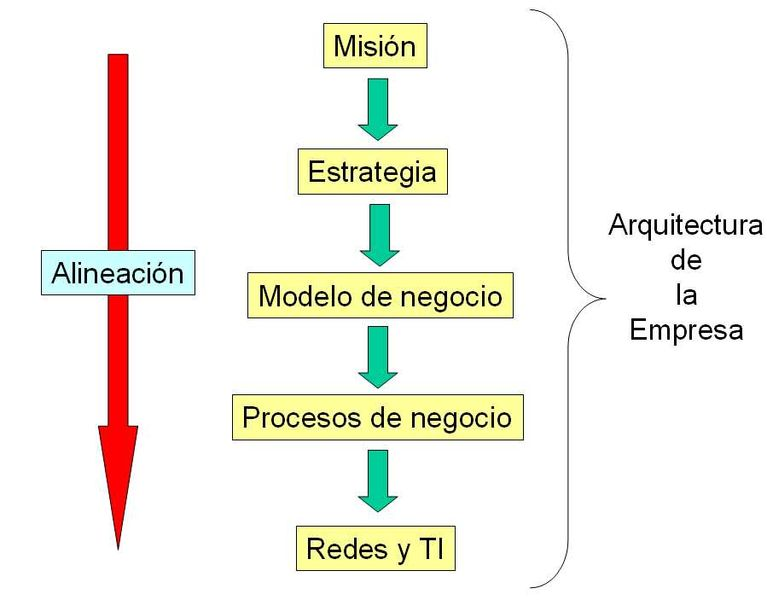
\includegraphics[height=8cm]{images/arqEmpresa}
\end{center}

\begin{itemize}
	\item \emph{Misión:}
		Este es el nivel más alto y explica por qué existe la empresa.
	\item \emph{Estrategia:}
		En este nivel se define qué es lo que se tiene que hacer para cumplir con la misión de la empresa. Se revisa la empresa
		y su entorno externo (es frecuente utilizar técnicas como el análisis SWOT) para decidir cual es el mejor camino para
		maximizar las ganancias dados sus recursos actuales y la posición de la competencia. Es importante tener una visión de
		largo plazo para no caer en la trampa de ganancias a corto plazo que comprometan el futuro de la compañía. Los modelos
		clásicos de competencia son los de Michael Porter: Diferenciación o Liderazgo en costos.
	\item \emph{Modelo de negocio:}
		Este nivel actúa como etapa de conexión entre el nivel Estratégico y el de Procesos de negocio (sin este nivel, la transición
		entre uno y otro es más difícil debido a la ambigüedad que genera el gran paso en el nivel de abstracción). Se explica cómo
		es que la empresa va a generar sus utilidades. Se debe documentar cómo es que las diferentes áreas se relacionan entre sí para
		generar valor para los clientes. Es común describir las etapas de Innovación del producto, Administración de relaciones con los
		clientes, Administración de la Infraestructura, y por último, los Aspectos Financieros (modelo de Yves Pigneur y Alexander
		Osterwalder).
	\item \emph{Procesos de negocio:}
		En este nivel se describen las actividades más importantes de la empresa (el núcleo del negocio). Se sugiere modelar la Cadena
		de valor del negocio y de ahí obtener los procesos del negocio. Los procesos son un conjunto de actividades relacionadas y
		agrupadas que en conjunto reciben un insumo y producen una salida. Dichos procesos pueden automatizarse mediante sistemas de
		cómputo desarrollados a la medida o mediante la compra de sistemas existentes en el mercado como ERP (Planeación de Recursos
		Empresariales) o BPM (Business Process Management)
	\item \emph{Redes y Tecnologías de la Información:}
		Esta etapa se refiere a la tecnología que debe utilizarse para apoyar los procesos de negocio. Claro está que toda la información
		contenida en cualquier tipo de sistema de cómputo no serviría de mucho sin redes de computadoras que permitieran la comunicación
		de dicha información entre clientes, proveedores y la empresa misma.
\end{itemize}
\newpage
